\subsubsection{Ažuriranje plana ishrane}

\begin{itemize}
    \item Kratak opis:
        \begin{itemize}
            \item Registrovani klijent ažurira svoj plan ishrane.
        \end{itemize}
    \item Učesnici:
        \begin{itemize}
            \item Registrovan klijent
        \end{itemize}
    \item Preduslovi:
        \begin{itemize}
            \item Klijent mora biti registrovan i ulogovan na aplikaciju.
            \item Klijent ima odabran plan ishrane.
            \item Prva sledeća dostava narudžbine je zakazana za dalje od pet dana.
        \end{itemize}
    \item Postuslovi:
        \begin{itemize}
            \item Podaci su uspešno sačuvani u bazi podataka, zakazana je dostava hrane i novac će biti skinut sa računa narednog dana.
        \end{itemize}
    \item Osnovni tok:
        \begin{enumerate}
            \item Klijent bira opciju da ažurira svoj plan ishrane.
            \item Sistem prikazuje klijentu formu za izmenu plana.
            \item Klijent ažurira i potvrđuje odabir plana.
            \item Sistem čuva podatke i skida novac sa klijentovog računa dan nakon što istekne mogućnost da menja svoj plan ishrane.
            \item Sistem prikazuje poruku o uspešnosti. 
        \end{enumerate}
    \item Alternativni tok:
        \begin{itemize}
            \item[4.a] Ukoliko sistem ne uspe da obavi skidanje novca sa računa, obaveštava klijenta o tome sa mejlom o grešci. Proces se nastavlja u 3. koraku osnovnog toka.
        \end{itemize}
    \item Dodatne informacije:
        \begin{itemize}
            \item Moguće je ažurirati recepte koji su izabrani, ažurirati tip plana(vrsta obroka, broj ljudi i broj obroka), ažurirati adresu, datum i satnicu dostave, preskočiti dostavu za ovu nedelju i otkazati pretplatu. 
        \end{itemize}
\end{itemize}

\begin{figure}[H]
\begin{center}
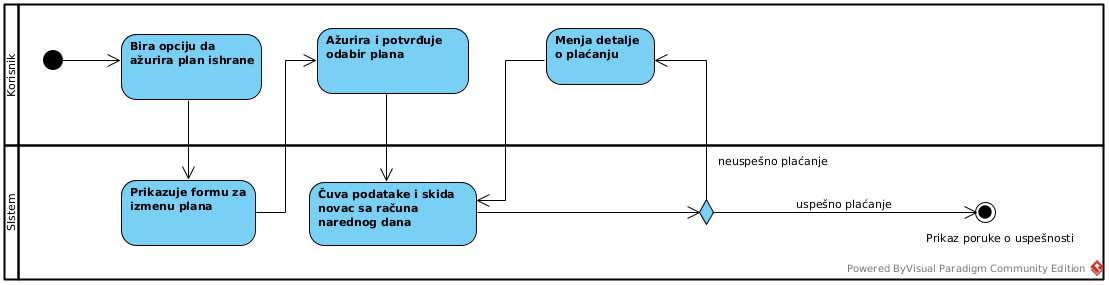
\includegraphics[width=\textwidth]{activity_update_meal_plan.png}
\end{center}
    \caption{Dijagram aktivnosti ažuriranja plana ishrane}
\label{fig:ActivityUpdateMealPlan}
\end{figure}
